\documentclass[12pt,a4paper]{article}
\usepackage[margin=1in,left=1.5in,includefoot]{geometry}
% Graphic
\usepackage{graphicx}
\usepackage{float}
% Hyperlinks
\usepackage[hyphens]{url}
\usepackage{hyperref}

% Header and footer
\usepackage{fancyhdr}
\pagestyle{fancy}
\fancyfoot{}
\fancyhead[LE,RO]{\bfseries\thepage}
\setlength{\headheight}{15pt}

% Quotes character
\usepackage[utf8]{inputenc}

% color links
\usepackage{color}  
\usepackage{hyperref}
\hypersetup{
    colorlinks=true, %set true if you want colored links
    linktoc=all,     %set to all if you want both sections and subsections linked
    linkcolor=black,  %choose some color if you want links to stand out
    urlcolor=blue
}

\begin{document}
\begin{titlepage}
	\begin{center}

\includegraphics[width=0.6\textwidth]{images/bordeaux.png}\\[1cm]


{\large Report}\\[0.5cm]	
	
	\line(1,0){400}\\[0.2in]
	\huge{\bfseries Land Use Classification in Remote Sensing Images by Convolutional Neural Networks}\\
	\line(1,0){400}\\[1.5cm]
	
	\noindent	
	
	\begin{minipage}[t]{0.4\textwidth}
		\begin{flushleft} \large
    	\emph{Authors:}\\
    	Xuan Thanh \textsc{Pham}\\
    	Manh Tu \textsc{Vu}
		\end{flushleft}
	\end{minipage}
	\begin{minipage}[t]{0.4\textwidth}
  		\begin{flushright} \large
    		\emph{Supervisor:} \\
    		Marie\textsc{Beurton-Aimar}
  		\end{flushright}
	\end{minipage}
	
	\vfill

% Bottom of the page
{\large \today}
	\end{center}
\end{titlepage}

% Front matter
\pagenumbering{arabic}

% Table content
\tableofcontents
\thispagestyle{empty}
\clearpage

% List of figures 
%\listoffigures
%\clearpage

\section*{Abstract}
In this project, we use the methods developed in the
article Land Use Classification in Remote Sensing Images
by Convolutional Neural Networks \cite{castelluccio2015land} to classify street images of the pagoda in Vietnam (Ho Chi Minh City). We collect the dataset from Google to train the network. After that, we try to experiment and analyze the result by testing our images of the pagoda which taking with our smartphones.

\section{Introduction}
\subsection{Image classification}
Image classification is the task of taking an input image and outputting a class which is a dog, cat, etc... or a probability of classes that best describes the image. For humans effortlessly to do the task of recognition, it comes naturally since we were born. But in computer vision, the computer must be trained in order to classify a set of data into different classes or categories. Training is the key to the success of classification.\\
\subsection{Convolutional Neural Networks}
Convolutional Neural Networks (ConvNets or CNNs) are a special type of Artificial Neural Networks. These models are designed to emulate the behavior of a visual cortex. CNNs perform very well on visual recognition tasks and has been some of the most influential innovations in the field of computer vision.\\
This model described in the article\cite{castelluccio2015land} as the most powerful in remote sensing datasets task. So, we're going to implement in our project in order to gain the best performance. 

\subsection{Caffe}

Caffe is one of the most popular libraries for deep learning (convolutional neural networks in particular). It is developed by the Berkeley Vision and Learning Center (BVLC) and community contributors. It supports the wide range of opera systems and graphical processing units in order to help us to train our model.\\
Caffe also makes easy to understand and configure our CNN layers. \\
In this project, we will use Caffe as our main deep learning framework.

\section{Task definition}
In order to classify street images of the pagoda in Vietnam (Ho Chi Minh City). We have to build a CNN model has an ability to recognize the photo of the pagoda which it has never seen before. \\
We also have to collect enough images of the pagoda for both trains and validates tasks.\\
Finally, after trained our model, we have to test its performance by the other datasets and build the web page to test our street images.

\section{Our solution}
\subsection{Dataset}
We found a MIT Computer Science and Artificial Intelligence Laboratory website \cite{mit} which is a scene-centric database called Places, with 205 scene categories. After downloaded 132Gb images, we built our own train dataset including:
\begin{itemize}
\item Pagoda: 15,100 images.
\item Not\_pagoda: 34,906 house images which are schoolhouse, courthouse and lighthouse. We chose those kinds of house because their building structure is a little bit similar with pagoda structure.
\end{itemize}

\begin{figure}[H]
\centering
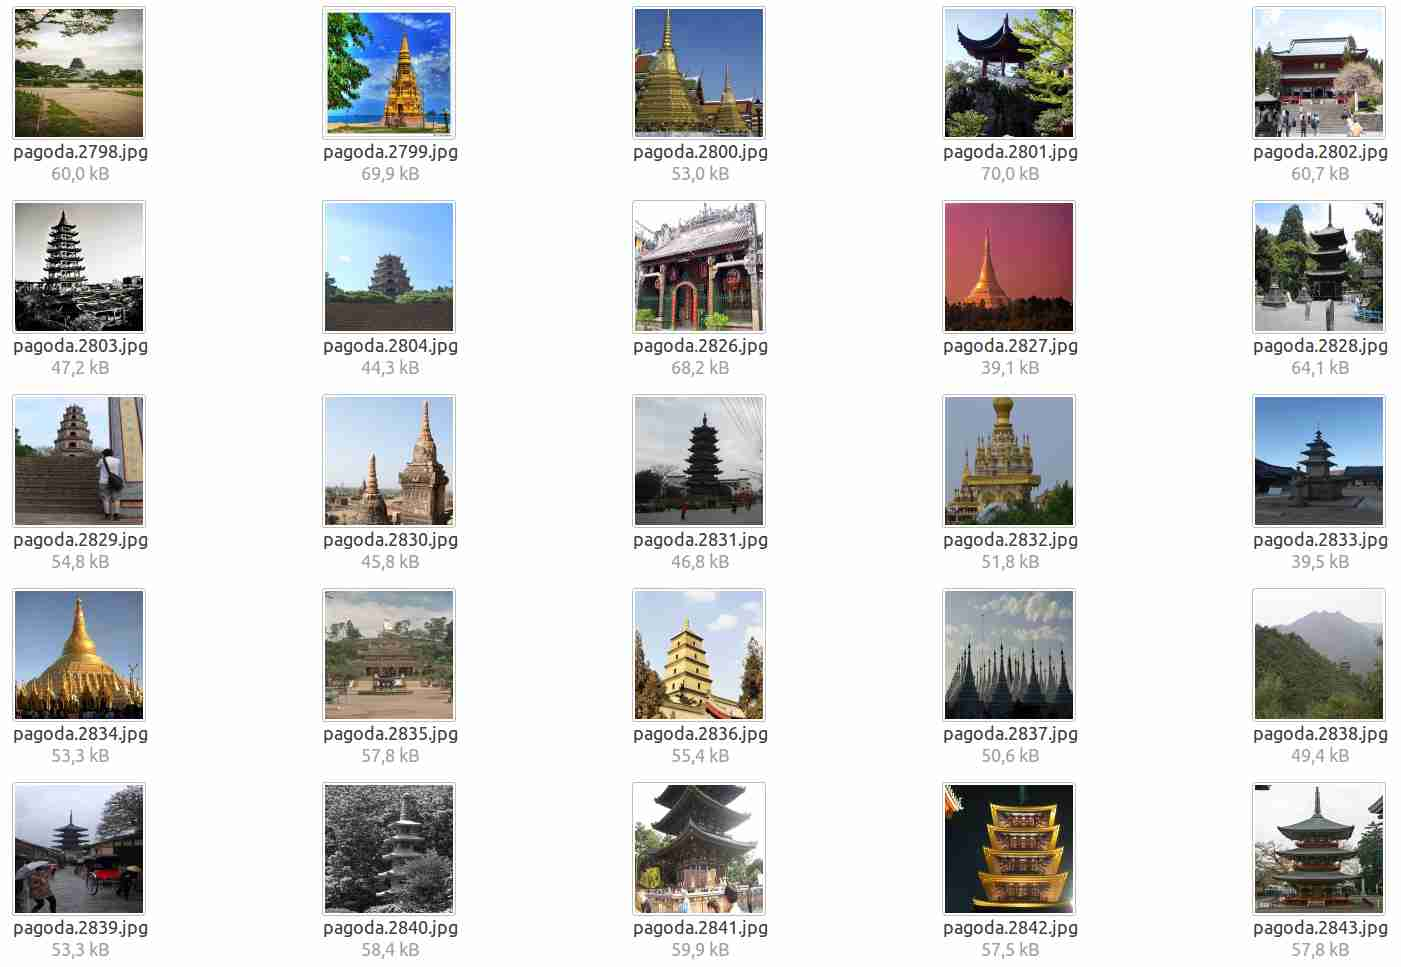
\includegraphics[width=1\textwidth]{images/sample.jpg}
\caption{Sample pagoda images of training dataset}
\label{fig:samplepagoda}
\end{figure}

\begin{figure}[H]
\centering
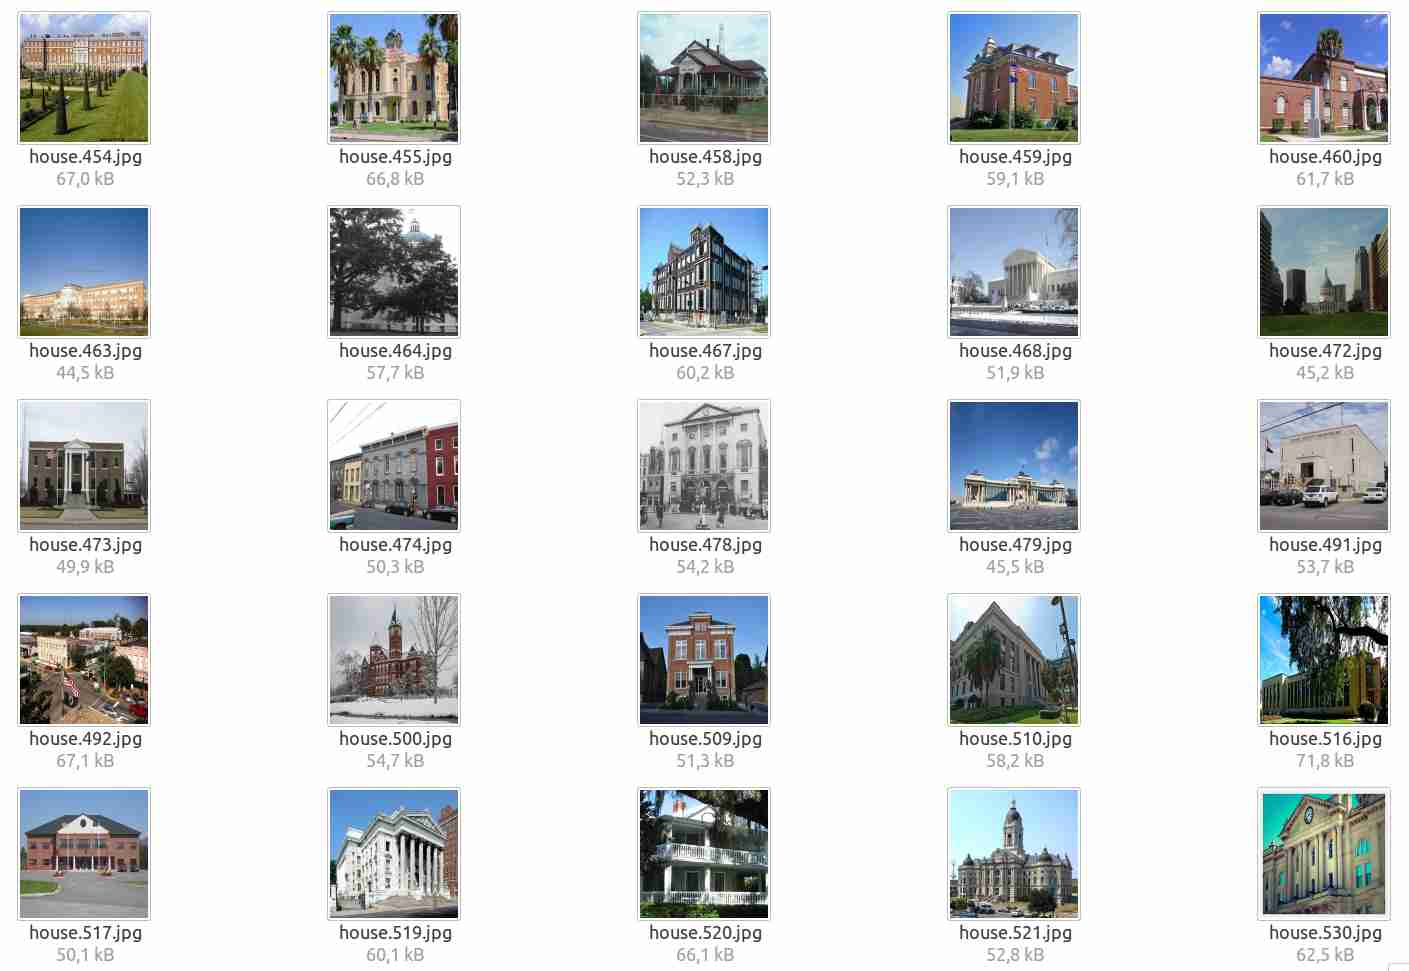
\includegraphics[width=1\textwidth]{images/sample2.jpg}
\caption{Sample not\_pagoda images of training dataset}
\label{fig:samplenotpagoda}
\end{figure}



\subsection{Hardware}
Because training CNN model with a large of dataset consumes a lot of time and resource, a standard PC or Laptop can't handle that. We already test our CNN model with a MacBook 2015 - Core i5 and 8GB Ram without external GPU. It takes about 12 hours for 200 iterators. This quite slow and our MacBook can't run forever.\\
To solve this problem, we hire an EC2 instance from Amazone Web Service\\
\\
\textbf{CPU:} Intel Xeon E5-2670 (Sandy Bridge) Processors\\
\textbf{GPU:} NVIDIA GRID GPUs, each with 1,536 CUDA cores and 4GB of video memory
\begin{center}
\begin{tabular}{| c | c | c | c | c |}
\hline
 Model & GPUs & vCPU & Mem (GiB) & SSD Storage (GB) \\ 
\hline
 g2.2xlarge & 1 & 8 & 15 & 1 x 60  \\
\hline
\end{tabular}
\end{center}

\subsection{Installing Caffe}
After some research, we found that currently, it has no completed script to install Caffe on Ubuntu 16.04 with Cuda 8 and CuDNN. It'll be difficult if we do it manually. So, to solve this problem and also help the other people who want to install Caffe, we decide to write a Bash script to automatic install Caffe with all dependencies, Cuda 8 and CuCNN under Ubuntu 16.04. You can see our topic at \href{https://github.com/BVLC/caffe/wiki/Caffe-installing-script-for-ubuntu-16.04---support-Cuda-8}{https://github.com/BVLC/caffe/wiki/Caffe-installing-script-for-ubuntu-16.04---support-Cuda-8}

\subsection{Data preparation}
Because of our dataset itself contain a lot of images, if we read them file by file, it can waste much time just because the limit of I/O. To solve this problem, Caffe using LMDB (Lightning Memory – Mapped Database) with high throughput. Our task is convert our dataset from stored to LMDB.\\

Before convert or dataset to LMDB, we use OpenCV to increase Histogram Equalization \& resize each images into 227x227 pixel. This help the Convolutional layer easy to recognize the different of the main object in the image.\\

We separate our dataset into two part, one is training (5/6) \& the other is validating (1/6). The validating help us to estimate how well our model has been trained and model properties (mean error for numeric predictors, classification errors for classifiers, recall and precision for IR-models etc.)\\

The last thing to do is computing image mean because the model requires us to subtract the image mean from LMDB we created before to improve detection accuracy.
\subsection{Model definition}
Our model is reuse from \href{https://github.com/BVLC/caffe/tree/master/models/bvlc\_reference\_caffenet}{bvlc\_reference\_caffenet} model, which is a replication of AlexNet with a few modifications.
The original bvlc\_reference\_caffenet was designed for a classification problem with 1000 classes. However, we just need to indentify if given image is pagoda or not. So, we change num\_output of the last InnerProduct layer from 1000 to 2.\\
We also change some information about location of mean image file, train \& validate lmdb in order to make the model work.\\
Finally, we have our model as describe in the image below:

\begin{figure}[H]
\centering
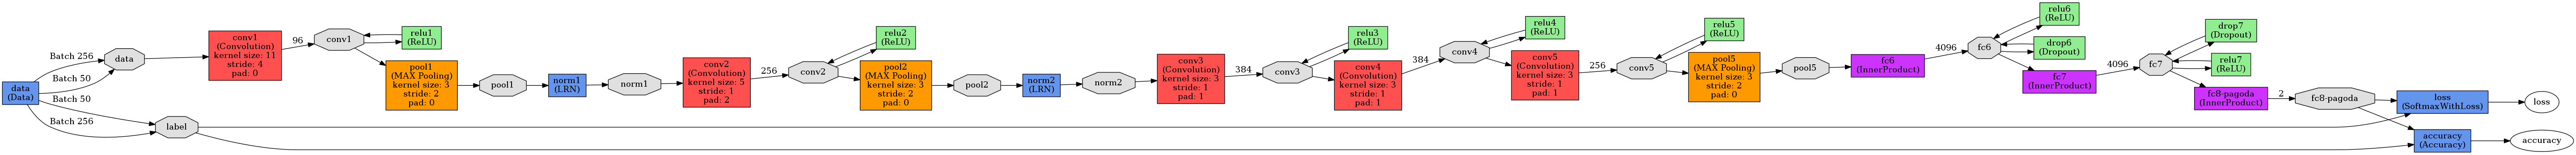
\includegraphics[width=\textwidth]{images/caffe_model.png}
\caption{Caffe model}
\end{figure}
\subsection{Solver definition}
Our model using Stochastic gradient descent solver method.
We run our model with 40.000 iterators, drop leaning rate every 2500 iterators and take a snapshot every 5000 iterators.
\subsection{Model training}
In order to reduce the time to train \& gain the best performance, we utilize the trained \href{https://github.com/BVLC/caffe/tree/master/models/bvlc\_reference\_caffenet}{bvlc\_reference\_caffenet} as a starting point of building our pagoda classifier using transfer learning. This model was trained on the ImageNet dataset which contains millions of images across 1000 categories\\
We used this fine-tuning strategy for training our model.
\section{Experimental}

\subsection{Plotting the Learning Curve}
A learning curve is a plot of the training and test losses as a function of the number of iterations. These plots are very useful to visualize the train/validation losses and validation accuracy. \\
We can see from the learning curve that the model achieved a validation accuracy of 98\%, and it stopped improving after 1000 iterations.
\begin{figure}[H]
\centering
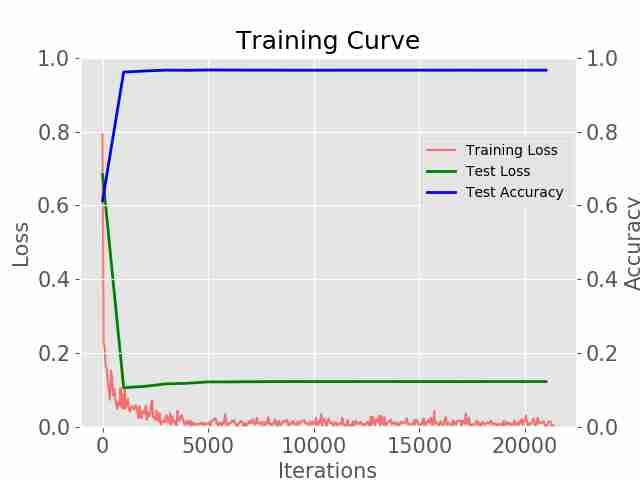
\includegraphics[width=0.8\textwidth]{images/trainningcurve.jpg}
\end{figure}

\subsection{Test performance}
To measure or CNN trained performance in a most objective way, we built the test dataset(1,519 images), which our CNN has never seen before. We collect the result after the test process \& compare with our expected result. Our dataset incudes:
\begin{itemize}
\item Pagoda: 999 images.
\item Not\_pagoda: 520 house images.
\end{itemize}
After train model, we test it with our dataset and get the accuracy 97\% (1,477 images is predict right, 47 images is not).
\begin{figure}[H]
\centering
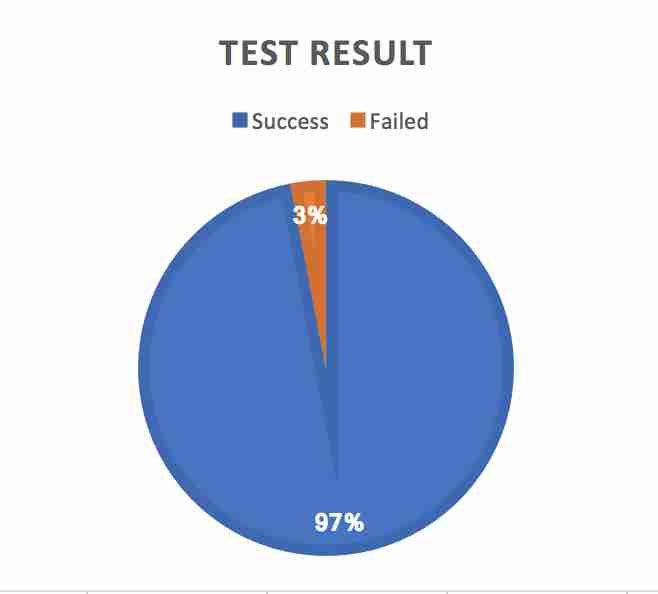
\includegraphics[width=0.8\textwidth]{images/testresult.jpg}
\label{fig:samplepagoda}
\end{figure}

\subsection{Resource}
\textbf{Testing page:} \url{http://54.255.219.234:8080/}\\
\textbf{Completed source code:} \url{https://github.com/glmanhtu/deeplearning-pagoda}\\
\textbf{Train dataset:} \url{https://drive.google.com/open?id=0B60FAQcEiqEyWlY1Uld-pVU5hT2c}\\
\textbf{Test dataset:} \url{https://drive.google.com/open?id=0B60FAQcEiqEyWUJ2dUh-mUDllb1k}\\
\textbf{Street image pagoda: } \url{https://drive.google.com/open?id=0B60FAQcEiqE-yRzBsYmFvZGNmRGs}

\bibliographystyle{plain}
\bibliography{bibfile}
\end{document}